\documentclass{bioinfo}
\copyrightyear{2015}
\pubyear{2015}

\begin{document}
\firstpage{1}

\title[Combined ChIP-seq discretization and quality control]{Zerone:
a ChIP-seq discretizer for multiple replicates with built-in quality control}
\author[Cusc\'o \textit{et~al}]{Pol Cusc\'o\,$^{1,2}$ and Guillaume
Filion\,$^{1,2}$\footnote{to whom correspondence should be addressed}}
\address{$^{1}$Genome Architecture, Gene Regulation, Stem Cells and Cancer
Programme, Centre for Genomic Regulation (CRG), The Barcelona Institute of
Science and Technology, Dr. Aiguader 88, Barcelona 08003, Spain.\\
$^{2}$Universitat Pompeu Fabra (UPF), Barcelona, Spain.}
% The CRG affiliation is compliant (October 17, 2015).

\history{Received on XXXXX; revised on XXXXX; accepted on XXXXX}

\editor{Associate Editor: XXXXXXX}

\maketitle

\begin{abstract}

\section{Motivation:}
Chromatin immunoprecipitation followed by high-throughput sequencing
is the standard method to investigate chromatin protein composition. As the
number of community-available ChIP-seq profiles increases, it becomes more
common to use data from different sources, which makes joint analysis
challenging. Issues such as lack of reproducibility, heterogeneous quality and
conflicts between replicates become evident when comparing data sets, especially
when they are produced by different laboratories.

\section{Results:}
Here we present Zerone, a ChIP-seq discretizer with built-in quality control.
Zerone is powered by a Hidden Markov Model with zero-inflated negative
multinomial emissions, which allows it to merge several replicates into a single
discretized profile. To identify low quality or irreproducible data, we trained
a Support Vector Machine and integrated it as part of the discretization
process. Zerone identified low quality data with 95\% accuracy. In terms of
performance, Zerone is more than 4 times faster than MACS for a similar
accuracy.

\section{Availability:}
Zerone is available as a command line tool and as an R package. The C
source code and R scripts can be downloaded from
\href{https://github.com/gui11aume/jahmm}{https://github.com/gui11aume/jahmm}.

\section{Contact:}
\href{guillaume.filion@gmail.com}{guillaume.filion@gmail.com}
\end{abstract}

\section{Introduction}
One of the major challenges of biology is to understand how transcription
factors and chromatin proteins coordinate genome-dependent processes
such as transcription, replication and repair. Massive research efforts
are invested into collecting protein-genome interaction data in order
to gain insight into the organization of the genome as a whole. Chromatin
immunoprecipitation followed by high throughput sequencing (ChIP-seq)
emerged as the standard method to identify the targets of a transcription
factor or a histone modification in a cell population. However, ChIP is not
fully understood and artifacts are still discovered more than 10 years after
its adoption \citep{pmid24349523, pmid24173036}. Besides, the constant
improvement of sequencing technologies makes analysis of ChIP-seq profiles
difficult to standardize. There is thus a continuous need to develop and
improve computational tools to analyse ChIP-seq data.

One of the most common analyses performed on ChIP-seq profiles is to
discretize the signal, \textit{i.e.} make calls whether the feature is
present or absent for every locus of the genome. This may seem
dubious at first glance because the biological reality is intrinsically
quantitative, but there are good reasons to discretize ChIP-seq
profiles: it makes the signal simpler to interpret from the human
perspective, it removes part of the experimental noise,
it simplifies downstream analyses and it allows to compare or
combine profiles of different nature. This raises a challenge at the
computational level because discretization has to be carried out uniformly
for signals that may have very different properties. For instance compare
the megabase scale domains of Lamin \citep{pmid18463634} to the 6~bp
binding sites of typical transcription factors.

Large consortia such as ENCODE have brought to light a more severe type
of issue related to the quality of ChIP-seq data. Conflicts between
replicates are common, and
sometimes laboratory effects are clearly detectable in the data,
even when experimentalists use the same material and follow the same
protocol (our unpublished observations). The most popular remedy is to
use a metric called IDR (Irreproducible Discovery Rate, \citealp{li2011}),
which allows to weed
out poorly reproducible signal. This approach is a significant step
forward, but the IDR is undefined when more than two replicates are
available. Besides, keeping only the reproducible ChIP peaks is not
always the best option. If one of the replicates is mislabelled,
for instance, it is more appropriate to reject the data set than to keep
the common ChIP peaks. In summary, how to integrate ChIP-seq data
from different sources and with variable qualities is still an open
problem.

Here we propose an approach to discretize ChIP-seq data where conflict
resolution and quality control are integrated in a tool that we called
Zerone. The key idea of Zerone is to combine an arbitrary number of
ChIP-seq replicates in a single discretized profile, where conflicts are
resolved by maximizing the likelihood of the underlying statistical model.
Following discretization, Zerone controls the quality of its output in
order to detect potential anomalies, and when applicable rejects the
output as a whole. Internally, the first step implements a Hidden Markov
Model (HMM) with zero-inflated negative multinomial (ZINM) emissions, and
the second implements a Support Vector Machine (SVM) trained using ENCODE
ChIP-seq data. HMM-based discretization is agnostic to the shape of the
signal (broad or peaky) and the ZINM distribution captures the essential
features of the read count distribution in ChIP-seq data. These two
properties provide a unified framework to discretize ChIP-seq data of
different kinds.

Zerone is designed for large volume pipelines aiming to combine many
ChIP-seq profiles with little human intervention. To this end, it is
compatible with the standard SAM and BAM formats \citep{pmid19505943},
it produces congruent window-based outputs, and it can process hundreds
of experiments per day on average hardware. We benchmarked Zerone against
MACS \citep{pmid18798982}, BayesPeak \citep{pmid19772557} and
JAMM \citep{pmid25223640} on the core
task of discretizing ChIP-seq profiles of CTCF, H3K36me3 and Pol2. Our
results show that Zerone is competitive in terms of speed and accuracy.

\begin{methods}
\section{Methods}

\subsection{Emission model}
\label{sub:emissions}
It is natural to model read counts in genomic windows by an unbounded
discrete distribution. The Poisson distribution is an obvious candidate,
but it is a poor choice because the variance of read counts is typically
higher than the mean in ChIP-seq data. The reason is that windows are non
homogeneous, which increases the dispersion. More specifically, windows
are not equally PCR-prone and not equally mappable. The negative binomial
(NB) distribution is thus a better choice because it allows some variation
between windows. However, genomes are fraught with repeats, which creates
an excess of windows where reads cannot be mapped. Since such windows
will always have 0 read count, a natural choice for this distribution is
the zero-inflated negative binomial (ZINB), \textit{i.e.} the mixture of
a negative binomial distribution and a distribution concentrated at 0.

The ZINB distribution has 3 parameters that can be fitted by maximum
likelihood. Zerone uses a custom solver based on the Newton-Raphson
method, which converges much faster than the popular routine
\texttt{zeroinfl} \citep{psclb} from the R \citep{R} package \texttt{pscl}
\citep{pscla}.
Fig.~\ref{fig:ZINB_fit} shows that the ZINB distribution gives a better
fit to ChIP-seq data than Poisson and NB distributions.

\begin{figure}[!tpb]
\centerline{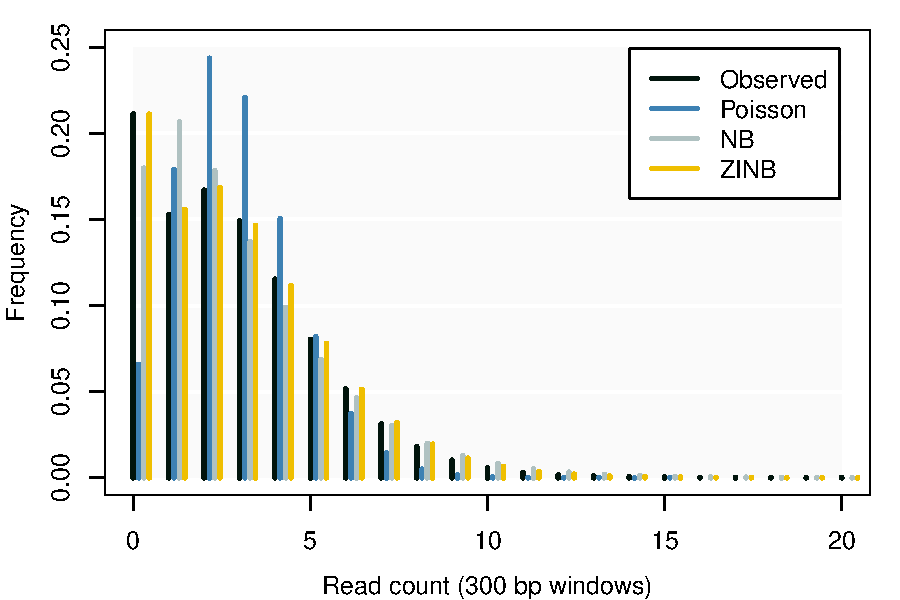
\includegraphics[scale=0.55]{ZINB_fit.pdf}}
% XX is wgEncodeSydhTfbsK562InputRawData.bed.gz %
\caption{
  Using the ZINB distribution to model ChIP-seq data. Reads from
  the negative control data set XX were mapped on the human genome and
  pooled in 300~bp windows after removing duplicates. The histogram of
  the read counts is shown in black (no immunoprecipitation was
  performed in this experiment, so this variation corresponds to the
  `baseline'). The histograms in gray scales show the maximum
  likelihood fit of the Poisson, Negative Binomial (NB) and
  Zero-Inflated Negative Binomial (ZINB) distributions. The fit of
  the Poisson distribution (light gray) is poor. The NB distribution
  (medium gray) gives a good fit at the tail, but not for windows with
  0 and 1 read. The ZINB distribution (dark gray) gives a good fit
  over the whole range.
}\label{fig:ZINB_fit}
\end{figure}

The NB distribution can be interpreted as a Gamma-Poisson process,
which gives a straightforward extension to a multivariate
distribution called the Negative Multinomial (NM) and to its
corresponding zero-inflated version the Zero-Inflated Negative
Multinomial (ZINM, see supplementary material for detail). In this model,
windows have an intrinsic ChIP-seq bias due to their sequence composition,
mappability and other inherent properties, which gives a baseline
variation present in all ChIP-seq experiments performed in the same
conditions. All the replicates of a ChIP-seq experiment can thus be
combined with the negative controls in a single multivariate
distribution.

\subsection{Discretization}
Discretization is performed by fitting an HMM
with ZINM emissions (see section \ref{sub:emissions}). The HMM has three
states corresponding to ``low'', ``medium'' and ``high'' abundance of
the given chromatin feature. We have observed that in many ChIP-seq
profiles, the baseline signal shows block-wise variations of low amplitude
but large size (typically 10-100 Kb). This will sometimes be the dominant
signal and a two-state HMM will identify these blocks instead of the
targets. Dedicating two states to fit the baseline is a way to make sure
that the ``high'' state corresponds to the targets of the chromatin
feature.

Fitting is performed with the Baum-Welch algorithm \citep{baum1966},
which is a special case of EM algorithm \citep{Dempster77maximumlikelihood}.
Discrete variables take only a small number of distinct values, which
allows to save computation time by hashing the observations. With this
technique, we need to compute each value of the emission probabilities
only once per cycle of the Baum-Welch algorithm. Transition parameters
are updated through the forward-backward algorithm, and emission
parameters are updated by solving maximum likelihood equations directly
with the Newton-Raphson method (see supplementary material for detail).
Approximately 3/4 of the computation time is spent in foward-backward
cycles, and 1/4 in updating emission parameters (the time spent computing
emission probabilities is insignificant). The algorithm stops when
parameters reach a stable value, or after a limit number of cycles (100
by default). The state calls are computed by finding the most likely
segmentation given the value of the parameters through the Viterbi
algorithm \citep{1054010}.

The shape parameter and the mixture ratio of the ZINM distribution
are fitted directly from the negative control profiles and they are
considered constant throughout. Overall, the total number of estimated
parameters is $3(r+1)$, where $r$ is the number of replicate experiments
(excluding negative controls).

\subsection{Classification and training}
\label{sub:training}
We used a machine learning strategy to identify discretization
failures. We first prepared a high confidence data set where the
output of Zerone was labelled positive (success) or negative (failure).
We discretized 144 replicated ChIP-seq experiments, together with their
respective input control.
We labelled the output for the discretization as positive (91 cases)
or negative (53 cases), based visual inspection and on the available
literature about the chromatin features. The most common cases of
poor data quality in ChIP-seq correspond to low signal-to-noise ratio
(\textit{e.g.} when the antibody is unspecific), and lack of
repdroducibility between replicates (\textit{e.g.} when samples are
swapped). To cover these cases, we included in the trusted set
38 other cases obtained by discretizing non-replicates
(\textit{e.g.} CTCF and Pol2) and controls without immuno-precipitation. Thus,
a total of 182 (91 positive and 91 negative) cases were used to build a balanced
dataset.

To identify discretization failures, we used the paremeters of the
fitted HMM. Based on the transition matrix, the emission paramaters,
the Viterbi Path and the posterior probabilities,
we computed 18 features expected to vary with the quality
of the discretization, and we used them to train a classifier.

Our first attempts with logistic regression suggested that linear
classifiers are unable to properly separate these two classes because
they overlap in the feature space (Fig.~\ref{fig:pca_bw}). To obtain more
complex, nonlinear separation, we used a Support Vector Machine
(SVM, \citealp{Chang2011,e1071}), as this approach guarantees the lowest
overfitting upper bound and allows nonlinear classification by mapping
the training data to a kernel space. Also, SVMs are fast to train and
they require only one hyperparameter to be fitted, which were
advantages over other approaches such as neural networks.

\begin{figure}[!tpb]
\centerline{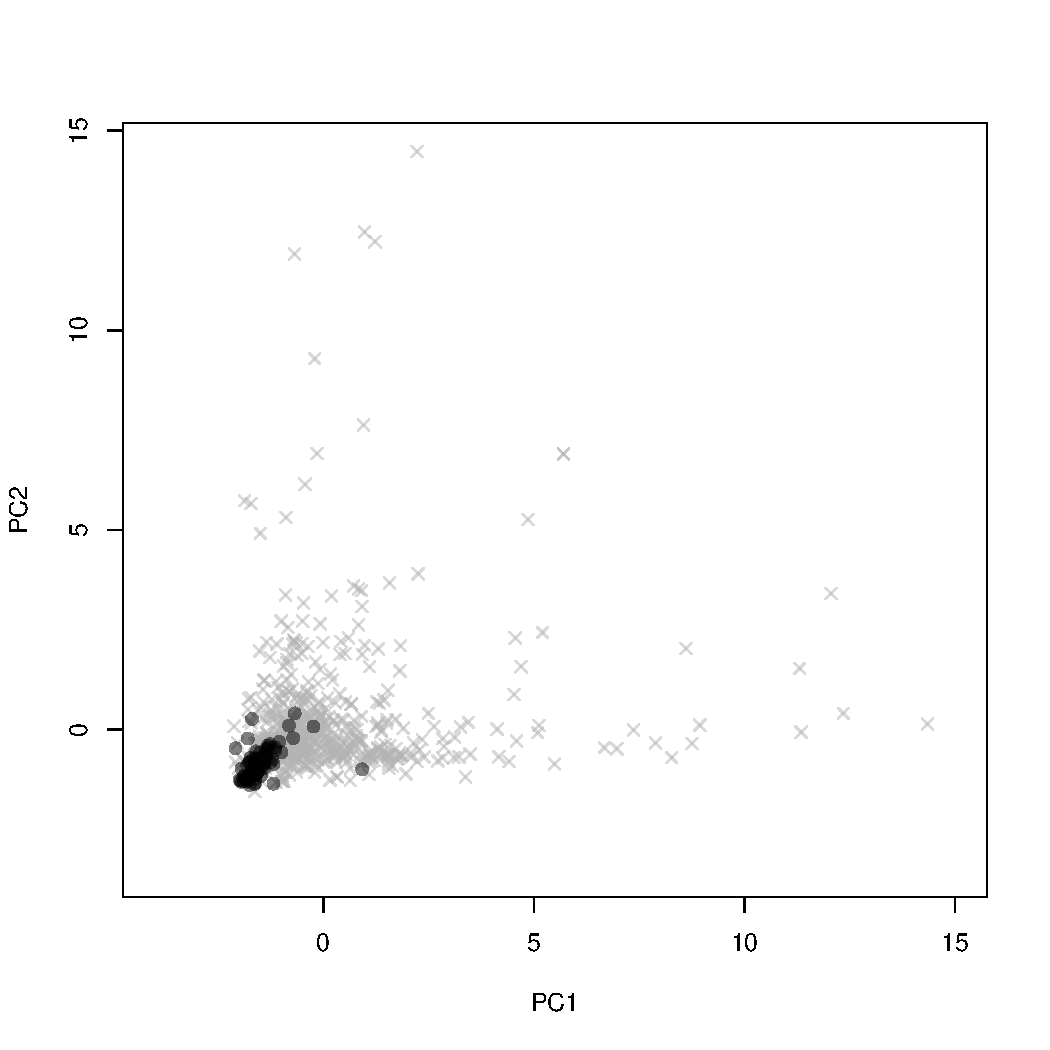
\includegraphics[scale=0.4]{pca_bw.pdf}}
\caption{
  Principal Component Analysis of the training data set.
  Each symbol represents a discretization performed by Zerone. The
  18 features extracted from each discretization are projected on the
  first two principal components. Positive examples (black circles)
  are similar to each other, while negative examples (grey crosses)
  are different from each other and from positive examples. The two
  groups overlap, which creates an ambiguous zone where failures and
  successes are indistinguishable.
}\label{fig:pca_bw}
\end{figure}

We trained the SVM with a radial basis function kernel and
selected the hyperparameters that maximized the prediction
performance on test sets using a 10-fold cross-validation scheme.
The prediction accuracy on the trusted set was 95\%.
We then implemented a prediction function in Zerone that used the
model trained by the SVM to classify the discretizations and
suggest whether they should be accepted or discarded.

\subsection{Datasets and preprocessing}
We used all the ChIP-seq profiles produced by the ENCODE consortium
on the human myelogenous leukemia cell line K562. We did not make use
of preprocessed mapped reads because they could have been mapped with
different software and could therefore disagree on its results
\citep{pmid21059603}. Instead, we mapped all the raw reads onto the
hg19 assembly of the human genome with GEM \citep{pmid23103880}, using
the options \texttt{--unique-mapping} and \texttt{-q ignore} of gem-mapper
version 1.376 (beta). The version of gem-indexer was 1.423 (beta). We
preprocessed the data in the same way both for training the classifier
and for benchmarking. We also used the same genome assembly to generate
the data sets used in the benchmarks (see Section \ref{sec:results}).

\subsection{Benchmark conditions}
To compare Zerone to other discretizers, we analysed three different
ChIP-seq data sets: CCCTC-binding factor (CTCF), tri-methylated histone H3 at
lysine 36 (H3K36me3) and RNA polymerase II (Pol2)---that represent punctate,
broad and mixed type signals respectively. Each data set consisted of an input
profile and two replicate target profiles.

To make the comparisons fair, we merged all contiguous windows that were called
as enriched by Zerone, in the same way the other programs do. Otherwise, the
number of enriched regions in the genome would be higher and Zerone performance
would look poorer than the actual.

We tested MACS \texttt{callpeak} version 2.1.0.20140616, BayesPeak
version 1.20.0 and JAMM version 1.0.7rev1. All tests were performed on
an 8-core Intel Xeon E5606 machine with 48~GB of DDR3-RAM at 1333~MHz.
All programs were run on a single core with the default options.

CTCF motifs were obtained from the JASPAR database version
5.0{\textunderscore}ALPHA \citep{pmid24194598}.

\end{methods}

\section{Results}
\label{sec:results}
We benchmarked Zerone against three other ChIP-seq discretizers.
We included MACS as the standard method for ChIP-seq peak calling,
BayesPeak because it is powered by an HMM with ZINB emissions
similar to the model implemented in Zerone, and JAMM because, as
Zerone, it can perform joint discretization of experimental replicates.

\subsection{Speed and memory footprint}

We compared the running times of the different programs on discretizing
three data sets of similar size that represent the three major types of
ChIP-seq signal usually observed. The CTCF signal consists of sharp
peaks at the transcription factor binding site, the H3K36me3 signal
consists of broad domains, and the Pol2 signal consists of  peaks
at promoters and potentially broad domains on transcribed genes.

The results were similar between experiments, and Zerone was
consistenty the fastest tool, with a running time around 5 minutes
(Fig.~\ref{fig:perf}, top row). The advantage is only marginal over
MACS, wihch ran for around 10 minutes, but it is substantial over
BayesPeak and JAMM, which ran in over 9 hours. The results for peak
memory usage were more variable between experiments (Fig.~\ref{fig:perf},
bottom row). MACS achieved the best performance with a memory
footprint around 0.5~GB, followed by Zerone around 1.0~GB.
BayesPeak and JAMM each used more than 1.5~GB.

The benchmark is partly confounded by the fact that BayesPeak and MACS
discretize a single input per run, whereas Zerone and JAMM discretize
multiple inputs simultaneously. This makes a difference for pipelines
where all files have to be processed in parallel with the minimum
amount of resources. In our benchmark, Zerone used twice as much memory
as MACS, but it also processed twice as many files. For the same amount
of available memory, a Zerone pipeline would run twice faster than a
MACS pipeline, and with only half the computer power.


\begin{figure}[!tpb]
\centerline{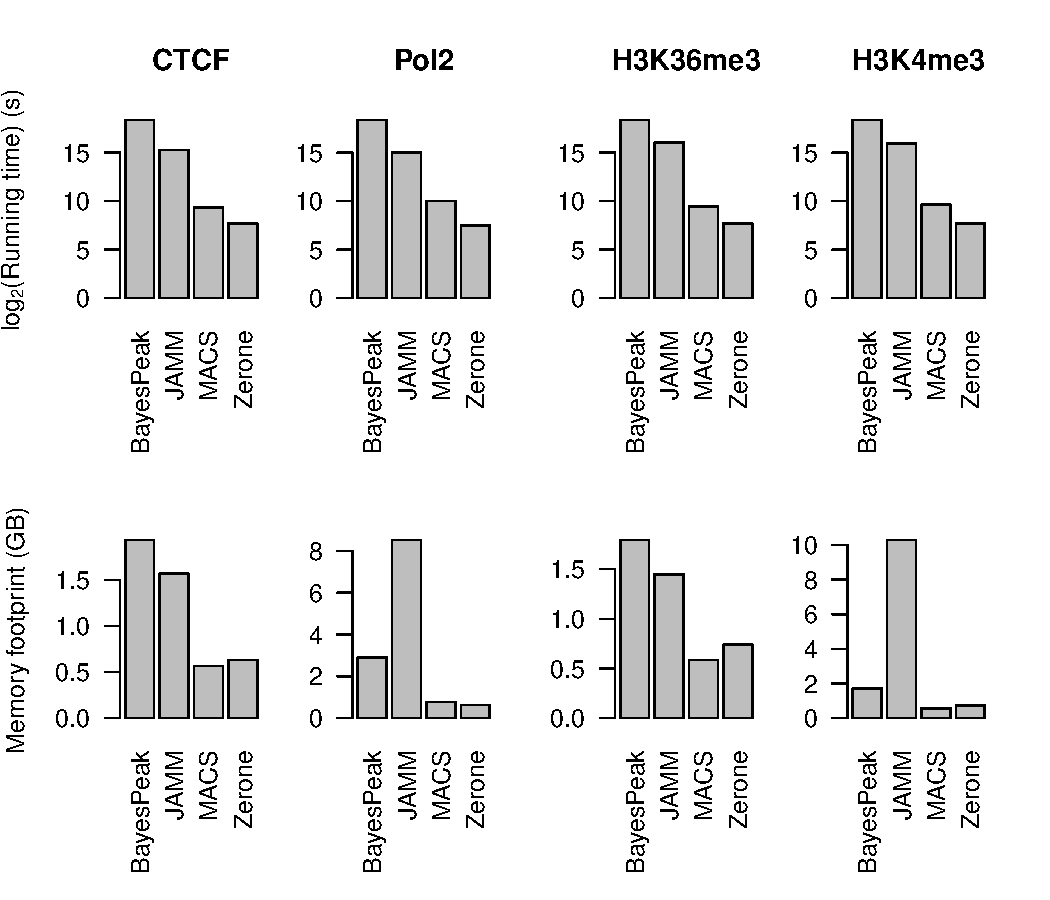
\includegraphics[scale=0.5]{performance.pdf}}
\caption{
  Running times and peak memory footprint of the
  discretizers on the three ChIP-seq data sets. For programs that only
  allow single-profile discretization (\textit{i.e.} BayesPeak and MACS),
  mean values (not the sum) are shown. Note the logarithmic scale in the
  running times.
}\label{fig:perf}
\end{figure}

\subsection{Accuracy}
The purpose of discretizers is to identify the targets of a
transcription factor or a histone mark, \textit{i.e.} the sites of
the genome where it is present.
Intuitively, good discretizers capture a large fraction of the
ChIP-seq signal within few targets. The number of targets
and the amount of reads they represent are therefore critical
characteristics of a discretization. Unfortunately, there is no gold
standard to estimate the trade-off between false positives and false
negatives in ChIP-seq experiments, and thus there is no objective way
to rank discretizers. However, we can compare them with a partial order,
as explained below.

\begin{figure}[!tpb]
\centerline{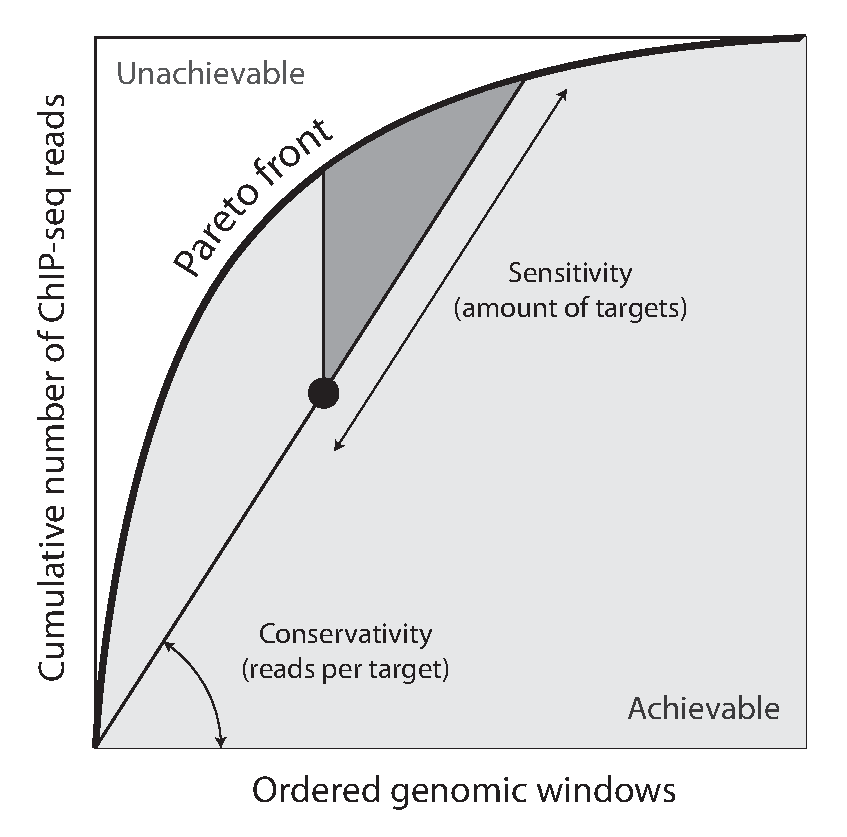
\includegraphics[scale=0.5]{pareto_front_explanation.pdf}}
\caption{
  Graphical representation of discretizations. Genomic
  windows of the ChIP-seq profile are ordered by decreasing amount of
  reads on the $x$ axis, and the cumulative amount of reads is plotted
  on the $y$ axis. This line forms a Pareto front representing the
  maximum number of reads for a given number of windows. Discretizations
  are represented as a single point on this plane (black disc) whose
  coordinates are the number of targets and the total number of reads
  in the targets. The dark triangle represents discretizations that
  are more conservative and discover more targets.
}
\label{fig:expl}
\end{figure}

When arranging genomic windows from high to low amount of ChIP-seq
reads, the cumulative number of reads forms a Pareto front.
It represents the largest amount of reads that can be captured by the
given amount of targets, or alternatively the smallest number of
targets that can catpure the given amount of reads
(Fig.~\ref{fig:expl}). A discretization can be represented as a point
on the $xy$ plane.  By construction, no discretization can lie on the
left of the Pareto front, and those on the front represent an
optimum. Others are suboptimal, since fewer windows can capture more
targets.

\begin{figure*}
\centerline{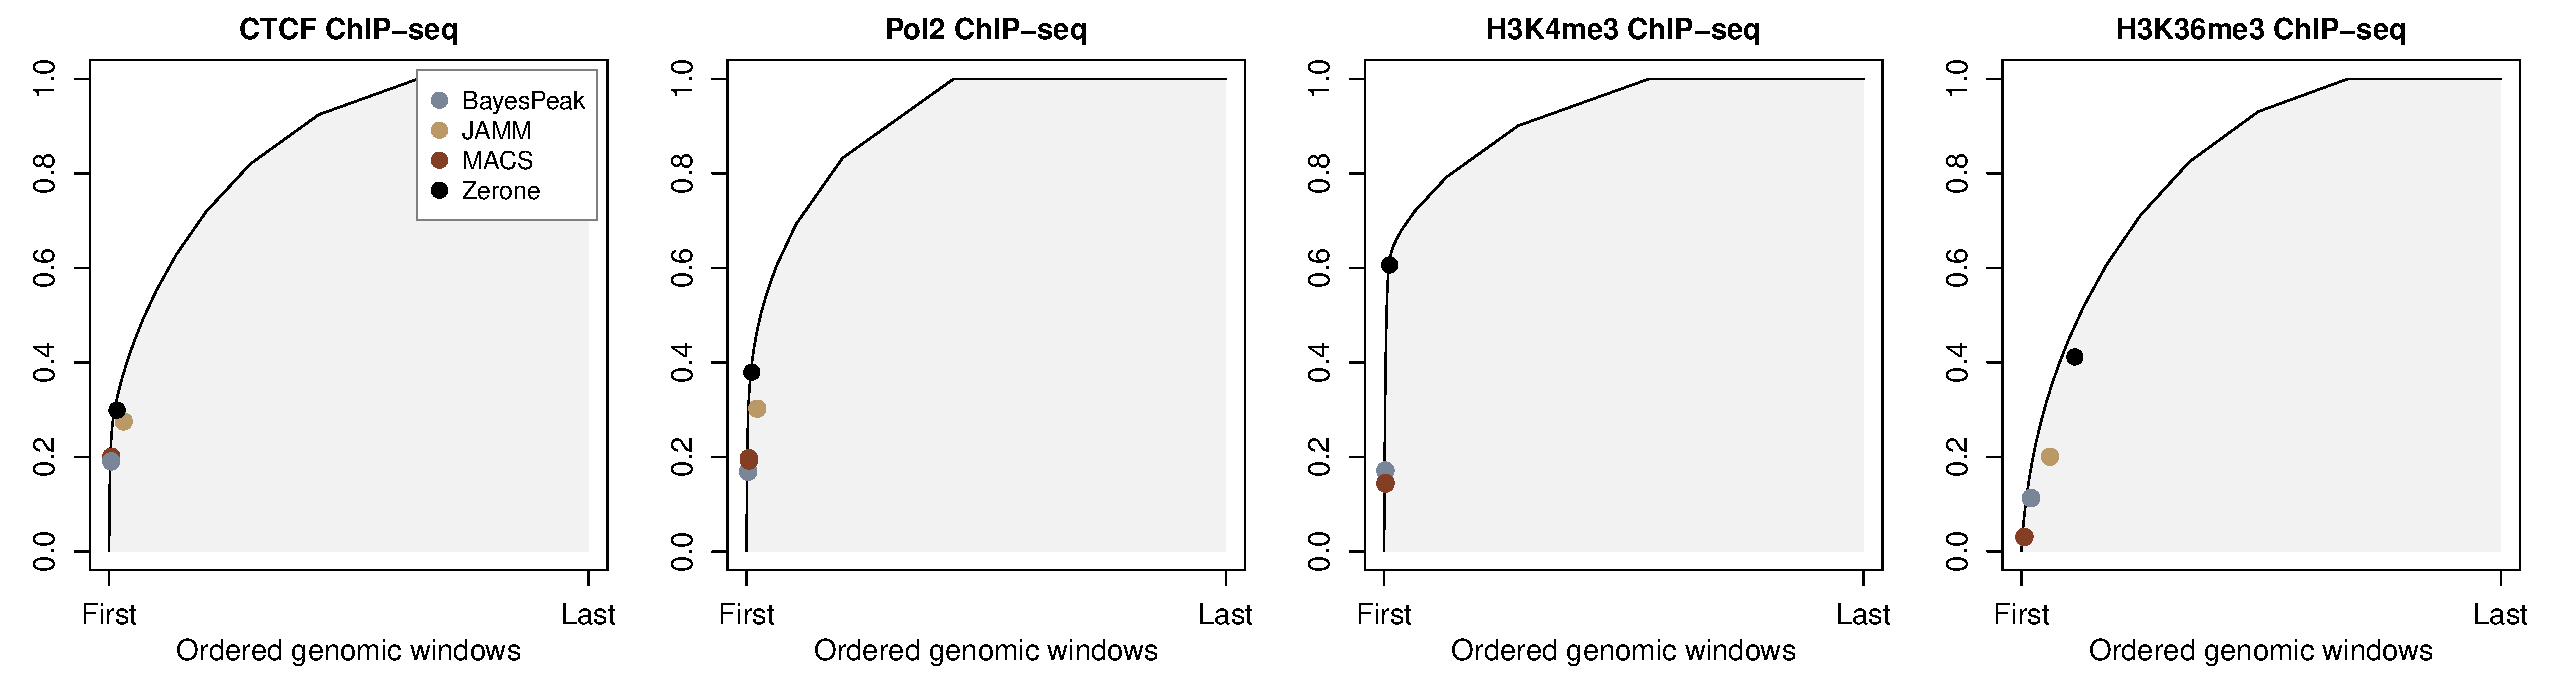
\includegraphics[scale=0.4]{pareto_front.pdf}}
\caption{
  Characteristics of the discretizations for different programs.
  The representation is obtained as shown on Fig.~\ref{fig:expl}.
  When discretizing the CTCF and the Pol2 profile (left and middle),
  Zerone produces discretizations that are very close to the Pareto
  front. In the case of H3K36me3, the discretization is off the
  Pareto front, but it is more sensitive and more sensible than the
  others.
}
\label{fig:pareto}
\end{figure*}

This representation reveals that discretizing the CTCF profile yields
similar outputs regardless of the software (Fig.~\ref{fig:pareto},
left panel). On the other hand, discretizing the Pol2 or the H3K36me3
profile yields very distinct outputs (middle and right panels). In
all the cases, Zerone produces the discretization capturing the most reads.
For CTCF and Pol2, it lies on the Pareto front at a kink of the curve,
\textit{i.e.} where the amount of reads per target starts to vanish. For
H3K36me3, it lies off the Pareto front, but at a sensible location.
Indeed, it has long been observed that histone modifications have more
ChIP targets than transcription factors \citep{XXX}. Of the other tools,
only JAMM produces a discretization that is consistent with those
facts.

This representation shows that Zerone produces discretizations that
are sensitive and adapted to the profile being discretized.


\subsubsection{Identification of CTCF binding sites.}
CTCF binds a 20~bp consensus sequence that is highly conserved in
vertebrates. In humans, nearly 80\% of the CTCF binding
sites contain the consensus motif \citep{pmid17382889}. In order to
determine the capacity of the different programs to call peaks of CTCF
binding, we compared the discretized profiles against a data set of CTCF
binding motifs. We used FIMO \citep{pmid21330290} from the MEME suite
version 4.10.1 \citep{pmid19458158} to identify and map CTCF motifs in
the human genome. We obtained a reference data aset containing 85,690
CTCF motifs.

Table \ref{tab:ctcf} shows that Zerone outperforms the other tools
in terms of the $F_1$ score (the harmonic mean between precision and
recall). It has a the second higest recall score, close to that of JAMM,
and it achievs the highest precision.

\begin{table}[!t]
\processtable{Performance on the CTCF motifs data set.
The table lists the total number of peaks found by the different
programs, how many of those peaks contain at least one CTCF motif,
and the associated precision, recall and $F_{1}$ score relative to
the CTCF motif data set.
\label{tab:ctcf}}
{\begin{tabular}{lrrccc}
        \toprule
        \textbf{Software}  & \textbf{Total}  & \textbf{Motif} &
        \textbf{Precision} & \textbf{Recall} & \textbf{$F_{1}$ score} \\
        \midrule
        BayesPeak$^{(1)}$ &  45,316 & 25,228 & 0.56 & 0.29 & 0.39 \\
        BayesPeak$^{(2)}$ &  45,154 & 23,428 & 0.52 & 0.27 & 0.36 \\
        JAMM              & 264,410 & 31,709 & 0.12 & 0.37 & 0.18 \\
        MACS$^{(1)}$      &  48,358 & 26,449 & 0.55 & 0.31 & 0.39 \\
        MACS$^{(2)}$      &  41,030 & 23,542 & 0.57 & 0.27 & 0.37 \\
        Zerone            &  50,792 & 30,972 & 0.61 & 0.36 & 0.45 \\
        \botrule
\end{tabular}}{The numbers in parentheses indicate the results on the two
replicates by separate.}
\end{table}

In summary, Zerone achieves a good balance between sensitivity and
specificity for transcription factor profiles, as was suggested by
the left panel of Fig.~\ref{fig:pareto}.


\subsubsection{Pol2 binding around transcription start sites.}
% Pol2 is on TSSs
To compare the behavior of the discretizers on the Pol2 profile,
we determined the extent to which the enriched regions contained Transcription
Start Sites (TSS), as Pol2 is expected to bind near annotated TSS. Data about
TSS positioning was extracted from the knownGene table of the UCSC Genes
annotation for the hg19 genome \citep{Karolchik2004}.

\begin{table}[!t]
\processtable{Performance on the Pol2 data set.
The table lists the total number of peaks found by the programs, how
many of those peaks contain at least one Transription Start Site (TSS),
and the associated precision, recall and $F_{1}$ score.
\label{tab:tss}}
{\begin{tabular}{lrrccc}
        \toprule
        \textbf{Software}  & \textbf{Total}  & \textbf{TSS} &
        \textbf{Precision} & \textbf{Recall} & \textbf{$F_{1}$ score} \\
        \midrule
        BayesPeak$^{(1)}$ & 208,809 & 2,722 & 0.01 & 0.06 & 0.03 \\
        BayesPeak$^{(2)}$ & 203,438 & 2,603 & 0.01 & 0.05 & 0.03 \\
        JAMM              & 209,882 & 6,761 & 0.03 & 0.21 & 0.11 \\
        MACS$^{(1)}$      &  51,313 & 6,845 & 0.13 & 0.22 & 0.27 \\
        MACS$^{(2)}$      &  49,034 & 6,546 & 0.13 & 0.21 & 0.26 \\
        Zerone            &  23,976 & 6,926 & 0.29 & 0.24 & 0.36 \\
        \botrule
\end{tabular}}{The numbers in parentheses indicate the results on the two
replicates by separate.}
\end{table}

Table \ref{tab:tss} shows that, as in the previous case, Zerone
achieves the highest $F_1$ score. Here it achieves both better
precision and better recall than the other discretizers, with a
very neat advantage in precision. These results confirm that
the performance of Zerone is outstanding on this dataset, as suggested
by the middle panel of Fig.~\ref{fig:pareto}.

\subsubsection{H3K36me3-enriched domains.}
Unlike the previous cases, there is no consensus sequence
to determine the location of histone modifications. However, it is
known that the bodies of active genes are enriched in H3K36me3
\citep{pmid16122420,pmid23739122}. Therefore, the genes that contain
peaks or windows determined as enriched in H3K36me3 by the different
discretizers should be more expressed than the background.

The majority of the enriched windows are detected by most programs.
This can be visualized in the Venn diagram of Fig.~\ref{fig:venn},
where Zerone is shown to be able to detect most of the windows detected
by other software, while discovering new enriched windows not found by
the others, which is consistent with the previous observations
(Table~\ref{tab:ctcf} and Fig.~\ref{fig:expr}).

\begin{figure}[!tpb]
\centerline{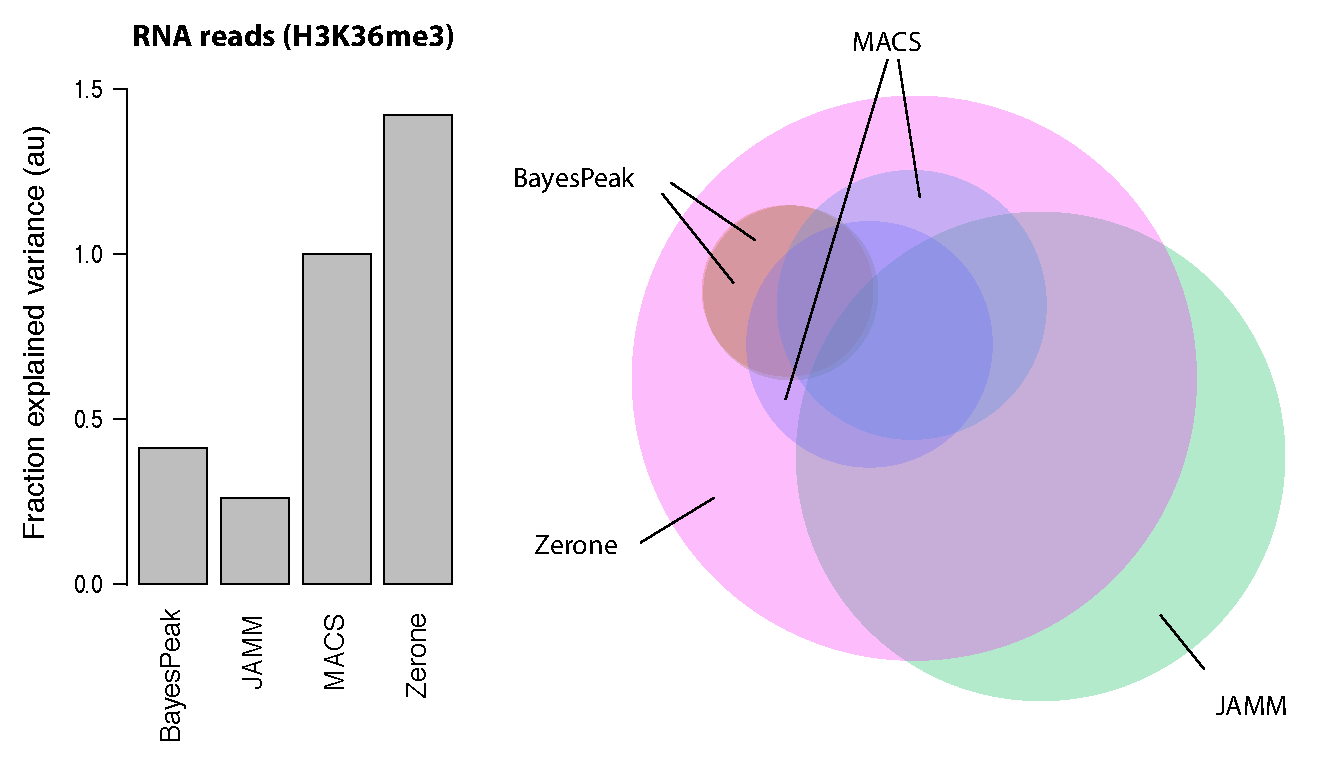
\includegraphics[scale=0.5]{histone_venn_color_names.pdf}}
\caption{Enriched genomic windows called by the different software.
Circle size represents the enriched portion of the genome according to
each of the programs, and the overlap between circles approximates the
amount of windows found enriched by two or more programs. Note the
almost complete overlap between the BayesPeak discretizations on the
two replicates.}\label{fig:venn}
\end{figure}

\subsection{Automatic quality control}

The most novel feature of Zerone is an embedded automatic quality
control step taking place after the discretization. This not only
ensures that the discretization is sensible, but also that the
replicates are similar to each other and that ChIP-seq profiles
are not too similar to the mock controls. Our approach is based
on the idea that estimating distributional parameters from
overly noisy or divergent profiles should give a signature that
can be picked up by a specially trained classifier.

We identified 18 summary statistics that characterize the
discretization (including the transition parameters of the HMM,
the mean number of targets and their mean posterior probability)
and trained an SVM to recognize failures. We thus obtained a
classifier able to identify failed discretization attempts
with 95\% accuracy (\textit{c.f.} section \ref{sub:training}).

Computer-assisted quality control is essential for high throughput
pipelines and for cases with no prior knowledge. We decided to
showcase this feature of Zerone on the ChIP-seq profile of HDAC6.
The issue with this protein is that it is almost exclusively
cytoplasmic, but that it is reported to have some enzymatic
activity in the nucleus \citep{XXX}. Is the amount of protein in
the nucleus sufficient to obtain good quality ChIP-seq profiles?

We used Zerone to discretize a ChIP-seq profile of HDAC6 in
K562 cells produced by the ENCODE consortium. The outcome of the
quality control is that the discretization is invalid. The
question is whether it is a botch of Zerone, or whether the data
is poor quality.

Find a ENCODE input that correlates well with the HDAC6.
If cannot, remove this section (or find another argument).

Do the fit of XXX signal with ZINB. Show that the signals are very
different.


\section{Discussion and conclusions}

Zerone was developed ground up for scalibility and throughput.
Part of the speed is due to indexing methods that dramatically
cut down the computation time during the Baum-Welch cycles. Zerone
also rests on sound statistical bases. Theoretical arguments and
experimental observations suggest that the Zero-Inflated Negative
Multinomial distribution is appropriate to model ChIP-seq data
(Fig.~\ref{fig:ZINB_fit}). This gives Zerone good specificity
and sensitivity for very different profiles.

Here we introduced a way to compare discretizers with an intuitive
grpahical representation (Fig.~\ref{fig:expl}). On this plane,
the coordinates of a discretization indicate the number of targets
(or occupancy) and the amount of reads captured by these targets.
The Pareto front captures the inherent trade-off between sensitivity
and specificity in the problem of discretizing ChIP-seq profiles.
Points on this line that are close to the bottom-left corner represent
discretizations with high amount of reads per target (most specific)
and points that are close to the top-right corner represent
discretizations with many targets (most sensitive). The Pareto front
also highlights an unachievable region whose shape depends on the
structure of the signal, \textit{i.e.} on the feature being disretized
(Fig.~\ref{fig:expl}). One of the challenges of discretizing ChIP-seq
profiles is to find algorithms that perform well in all the cases.

In practice, the specificity of a discretizer is unknown because
the biological truth remains hidden. However, we can decide whether
a discretizer is more or less conservative than another by measuring
the amount of reads per target. This characteristic may be a matter of
choice, and is usually tacit in the case of ChIP-seq discretizers.
Out of two equally conservative discretizers, one may be more sensitive,
\textit{i.e.} discover more targets. The merit of the representation
introduced here is to highlight these characteristics and to guide users
when choosing the most appropriate tool fo their need.

This representation naturally suggests a naive approach to discretize
ChIP-seq profiles. Indeed, one could sort the genomic windows by
decreasing amount of ChIP-seq reads and declare `target' any window
above a chosen threshold. While this method would only produce
discretizations on the Pareto front, adjusting the threshold to the
conditions would be challenging for lack of an underlying model.
This is one of the major strengths of Zerone: the statistical model
automatically adjusts conservativity and sensitivity in a sensible way.

\section*{Acknowledgement}

\paragraph{Funding\textcolon}
% These acknowledgements are compliant (October 17, 2015).
The fellowship of P.C. is partly financed by the Spanish Ministry
of Economy and Competitiveness (State Training Subprogram: predoctoral
fellowships for the training of PhD students (FPI) 2013).
We acknowledge support of the Spanish Ministry of Economy and
Competitiveness, `Centro de Excelencia Severo Ochoa 2013-2017',
SEV-2012-0208.

\bibliographystyle{natbib}
\bibliography{document,extra}

\end{document}
